\chapter{Background and Rationale}

\section{Background}

This project aims to create a serious game based on a robot in a remote laboratory. Moreover, it
aims to create a complete visual programming experience to teach the basics of programming. Thus,
in this state of the art, We will cover the three main topics that the project uses as a base and we
will deepen into them.

\subsection{Remote Laboratories}

Remote laboratories are usual laboratories, with the peculiarity that they can be accessed through
the Internet~\cite{remote_labs}. They give students the option to use the laboratory even from home
or while the university or school is closed. This means that the students are able to do their
homework or experimentation using the equipment at their school or university without the need for
them to be physically there.

Currently they are becoming more popular due to the competitive advantage they can give to schools
and universities. Since there is no need for the student to be physically in the laboratory, the
laboratory does not need to be physically in the school or university, giving the option to share
laboratories between institutions and thus giving important economic benefits without reducing
the practice time of the students, or even increasing it.

Thus, remote laboratories can be really helpful in teaching main concepts about science and
technology. The next laboratories are the most known ones that are working with science and
technology.

\subsubsection{Global Online Laboratory Consortium}

The \acrlong{golc} or \acrshort{golc} is an organization that focuses on the promotion of the
development of remote laboratories for educational use. They commonly promote remote laboratories
through conferences~\cite{golc1st}. They also support and encourage the sharing of these
laboratories between institutions.

For promoting laboratories, they created an award (Figure~\ref{fig:golc_award}) for remote
experimentation and another one for simulated experimentation.

\begin{figure}[!htbp]
	\centering
	
\includegraphics[width=0.5\textwidth]{fig/golc_award}
	\caption{\acrshort{golc} Online Laboratory Award 2015}\label{fig:golc_award}
\end{figure}

\subsubsection{WebLab-Deusto}

WebLab-Deusto is a remote laboratory located at the University of Deusto, Bilbao. There are multiple
types of laboratories there, and all is being controlled by a software they developed, called
WebLab. Moreover, Pablo Orduña, one of it's main researches developed a complete federation model
to be able to share laboratories across the world~\cite{porduna_phd}.

In WebLab-Deusto they created one of the most used remote laboratories in electronics teaching. It
is called \acrshort{visir}~\cite{visir}, and it recreates circuits made visually by students in real
hardware so that students can take real measurements.

\begin{figure}[!htbp]
	\centering
	
\includegraphics[width=0.5\textwidth]{fig/weblab}
	\caption{WebLab-Deusto logo.}
\end{figure}

\subsubsection{iLab Project at \acrshort{mit}}

The \acrlong{mit} has its own remote laboratory platform called iLab. They
have many remote laboratories where they experiment with Dynamic Signal Analyzers, Heat Exchangers
and even with Polymer Crystallization. It has even inspired some big projects using this technology
such as an on-line repository to locate remote laboratories~\cite{ilabs_multi}.

\begin{figure}[!htbp]
	\centering
	
\includegraphics[width=0.5\textwidth]{fig/icampus}
	\caption{iCampus logo, project at \acrshort{mit} where iLabs have been created.}
\end{figure}

\subsubsection{Robotic remote experiments}

Some of the laboratories listed before have currently implementations of robotic experiments in
as a teaching material in some areas. In WebLab-Deusto, for example, they have what they call
WebLab-Bot (Figure~\ref{fig:weblab-bot}). This robot is based on Azkar-Bot robot and it is used for
electronic students to learn how to program it. They have simple demonstrations that follow a black
line or respond to simple commands.

\begin{figure}[!htbp]
	\centering
	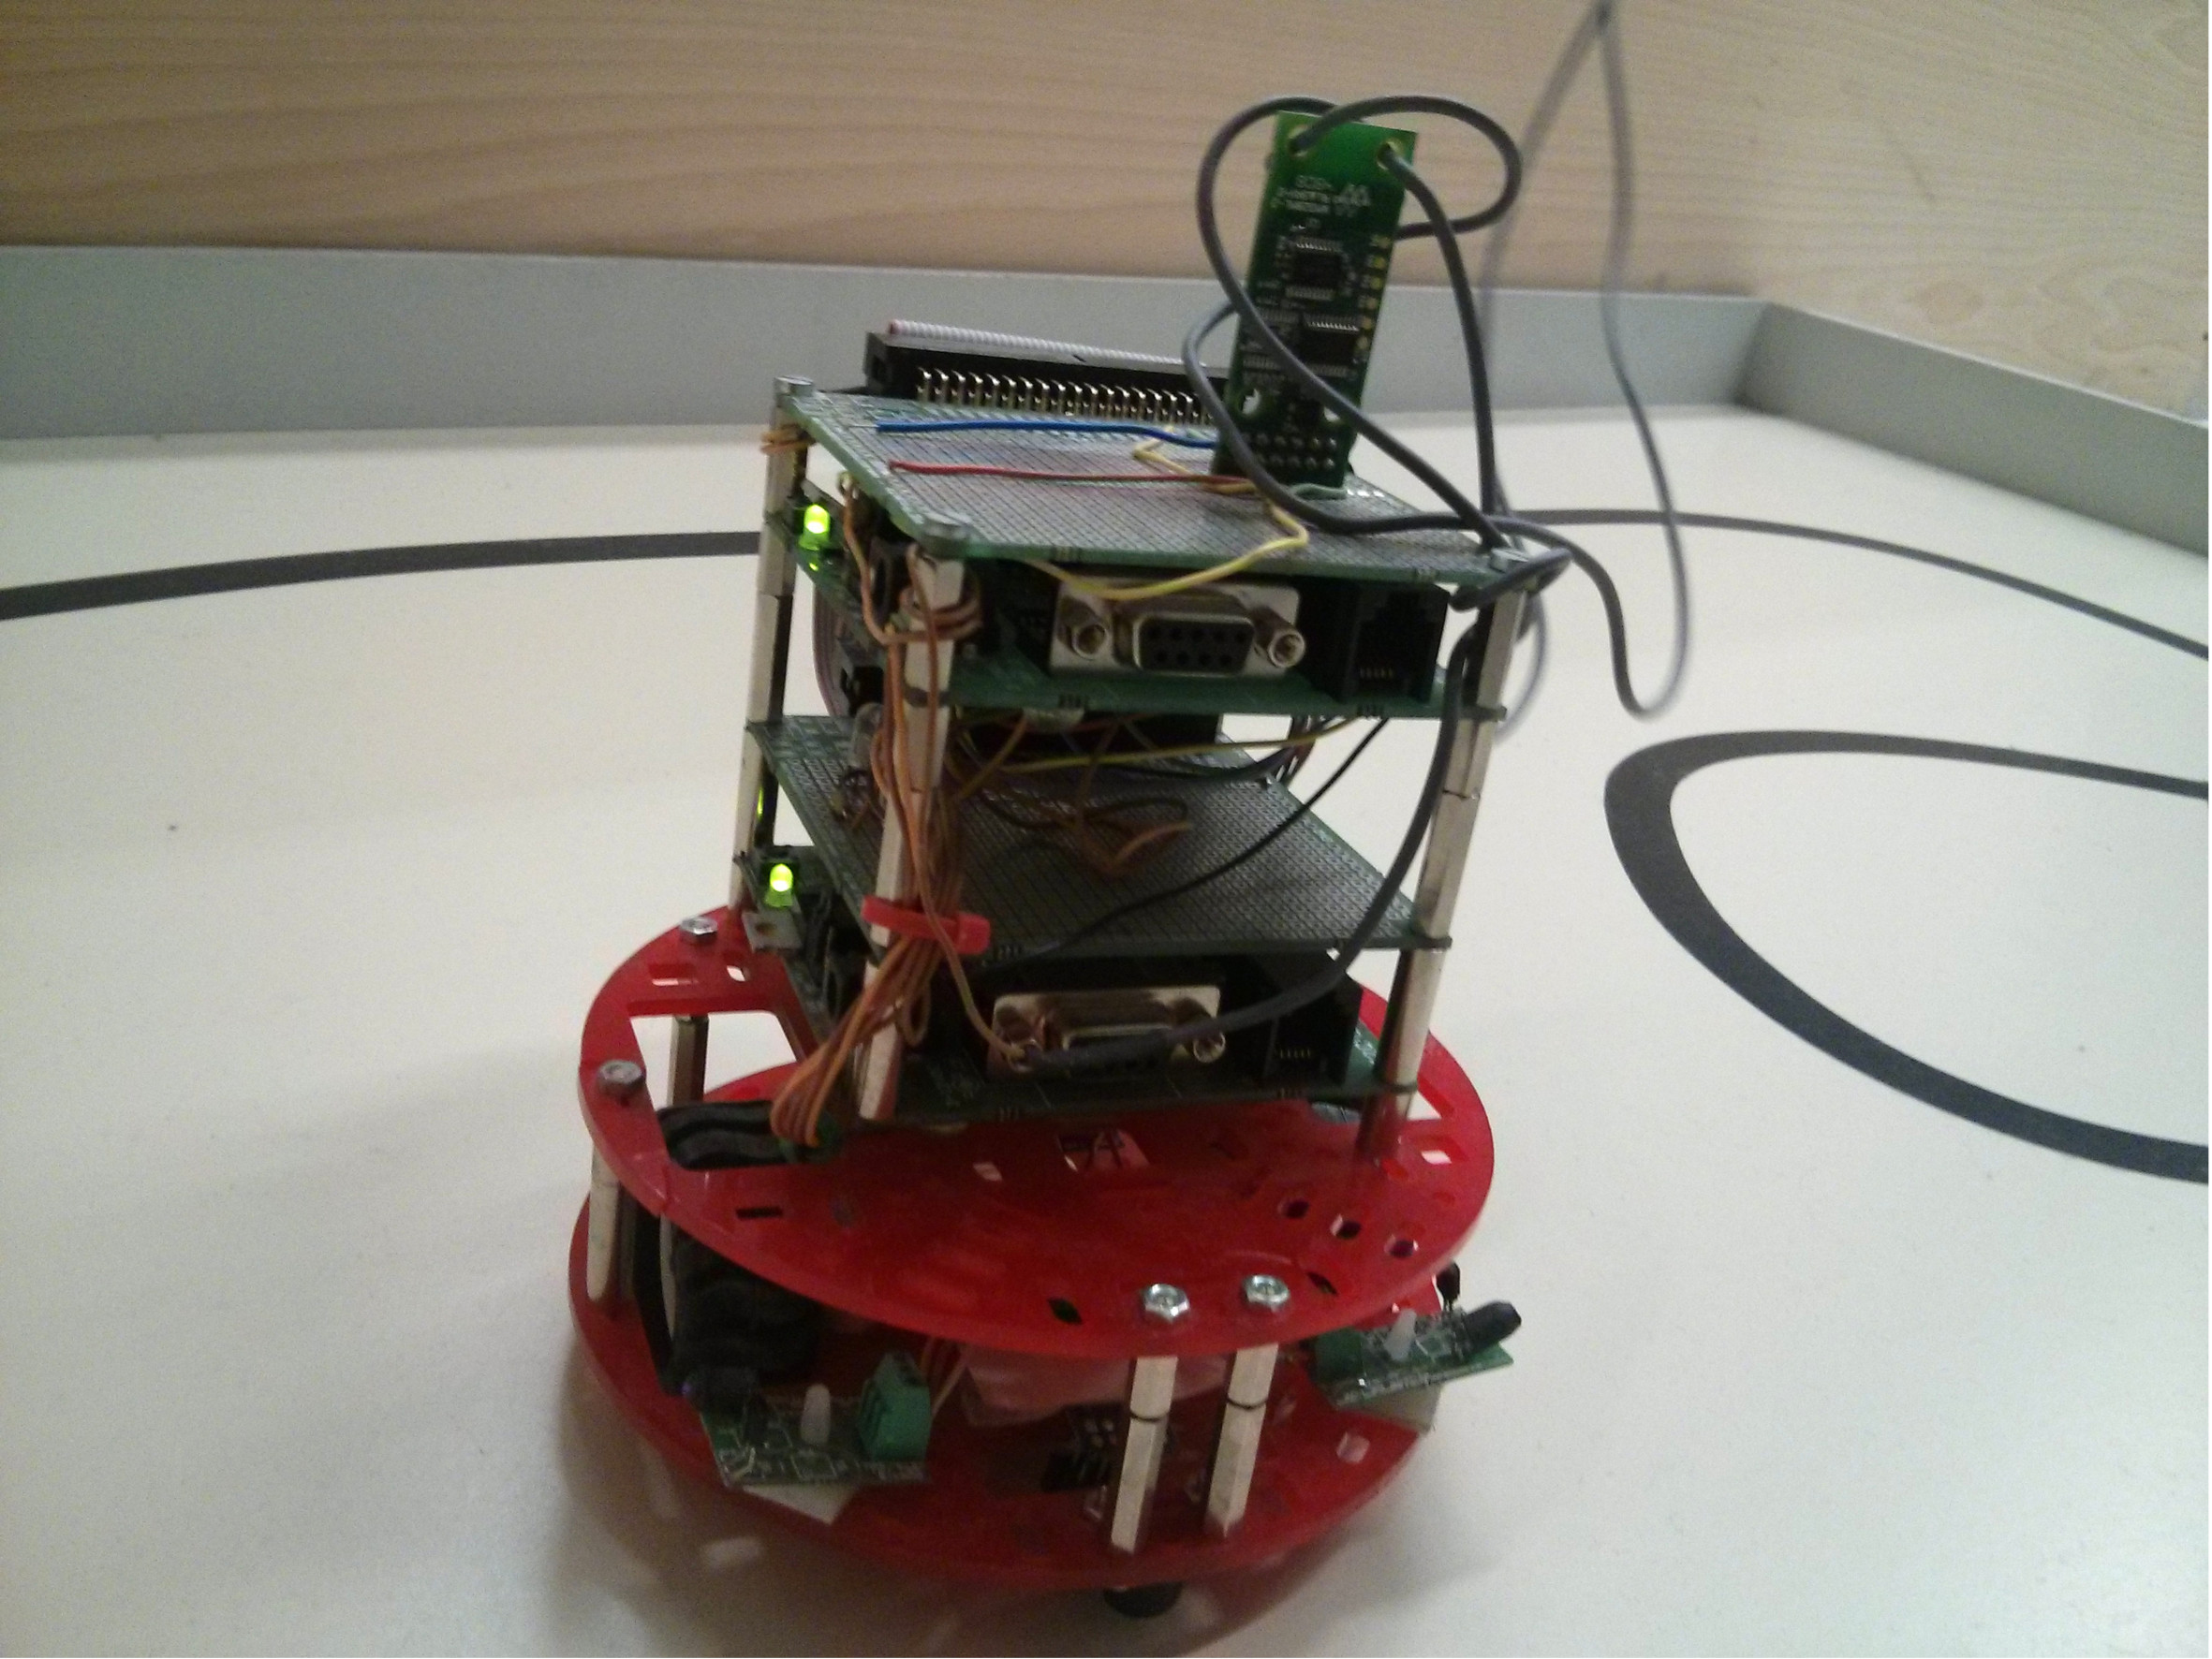
\includegraphics[width=0.5\textwidth]{fig/weblab-bot}
	\caption{WebLab-Bot, a robot based on Azkar-Bot as a remote laboratory in
	WebLab-Deusto.}\label{fig:weblab-bot}
\end{figure}

Moreover, in The Labshare Institute, they have a robot called iRobot, that teaches how to deal with
accuracy of sensors, localization and mapping. Finally, the robot that will be used in this
project is called Romie (Figure~\ref{fig:labyrinth}. It is located in WebLab-Deusto and it has the
needed functionality for this project: it is capable of following a line, it detects walls and it
detects intersections. We have built a complete labyrinth for it where we will deploy this project.

\begin{figure}[!htbp]
	\centering
	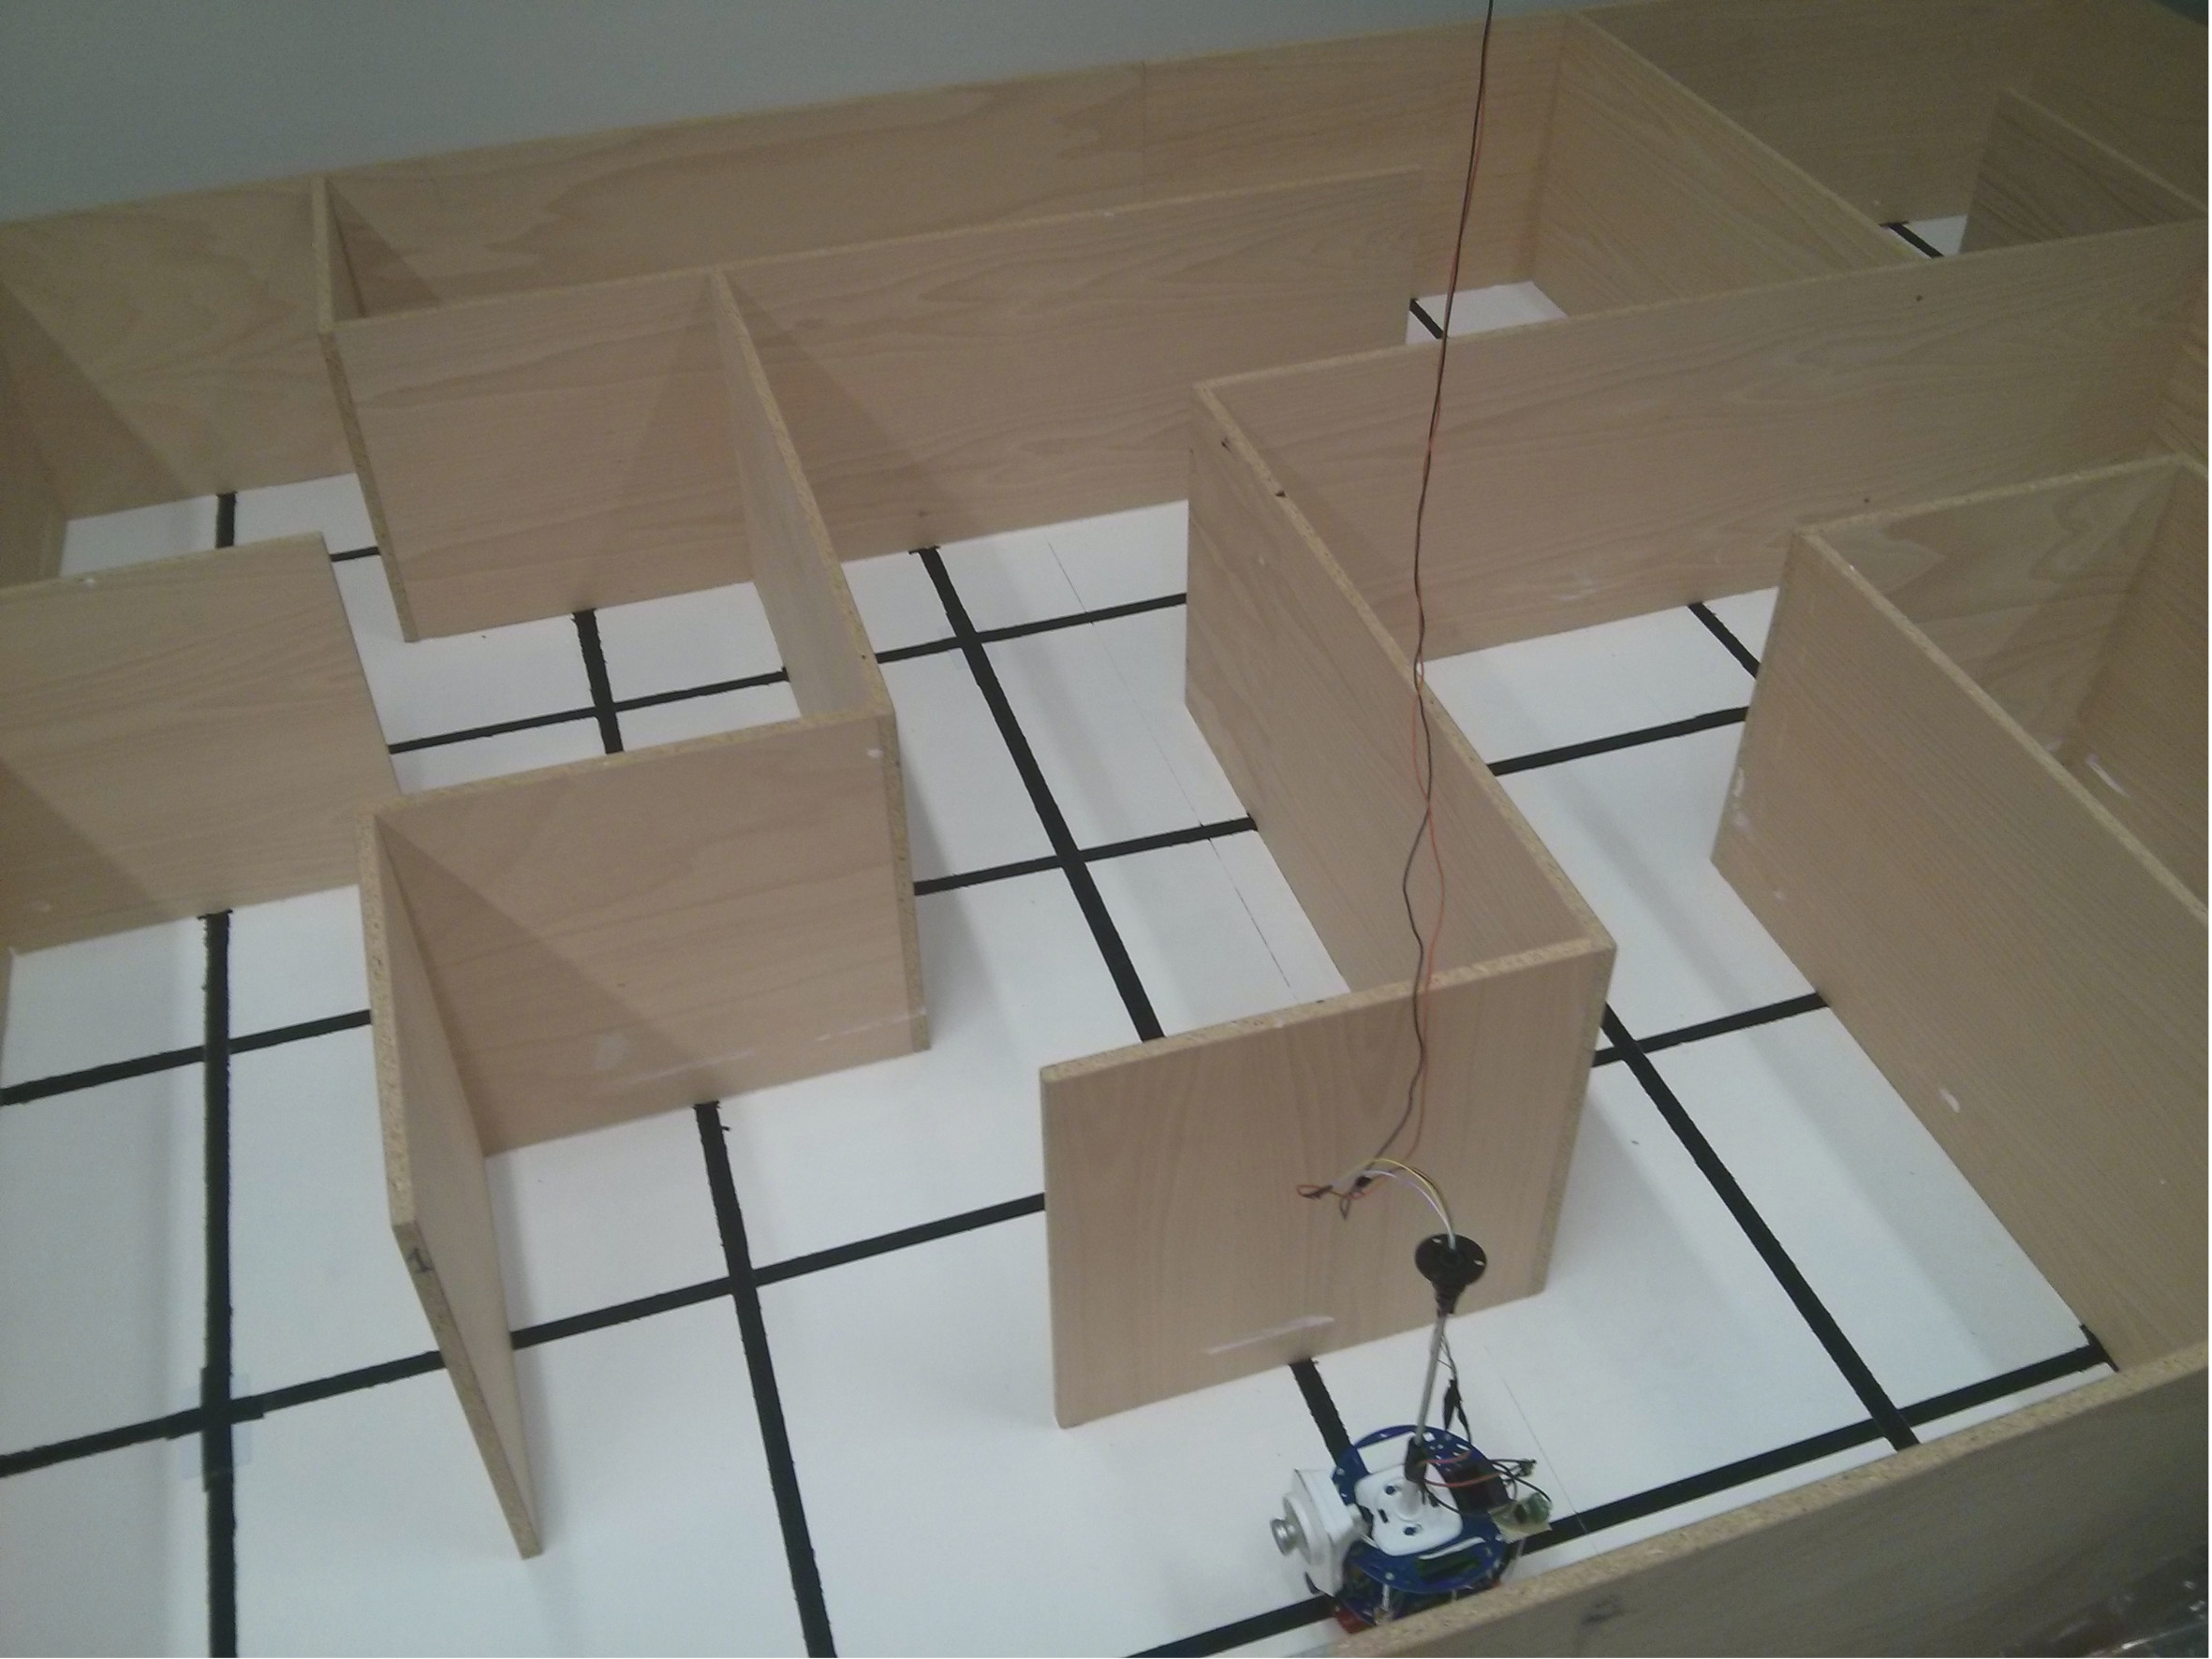
\includegraphics[width=0.5\textwidth]{fig/labyrinth}
	\caption{Romie, the robot we will be using in this project in its labyrinth.}\label{fig:labyrinth}
\end{figure}

\subsubsection{Simulations}

Even if the project will not be based on simulated robotics but in real robots, currently many
many projects use simulations to bring some of the experience to users. A simulation is usually
less costly than a remote laboratory, since not much hardware is required. On the other hand,
students will not be using real tools and experimentation environments, so the experience of using
them will not be as complete as in a remote laboratory.

Nevertheless, some prefer creating hybrid laboratories~\cite{hybrid_labs}. In these cases, the
laboratories add a simulation layer over the real laboratory. This way, the user still uses a real
laboratory, with the benefits of knowing how to use the laboratory and doing real experimentation,
and it also gives the user some more benefit by simulating extra conditions that could be expensive
to create in a real laboratory.

\subsection{Serious Games and Visual Programming}

Serious games are video games that do not only entertain, but they manage to teach. Thanks to that,
they can be used to improve the quality of the learning environment for students. Moreover, since
games in many cases attract better the attention of young people, they can even be a better tool for
teaching, at least, the basic concepts of some subjects. For our purpose here, we will analyze the
most known tools for visual programming environments.

Visual programming is a way of programming that instead of using real code in a real programming
language uses a visual interface to create programs and then translate them to a well known
language. This way, people that are not yet used to programming languages, interfaces such as IDEs
or code execution, and do not understand the basis of programming can start learning by using a
simple visual environment~\cite{visual_programming}.

\subsubsection{Scratch}

Scratch is one of the most known visual programming tools~\cite{scratch}. It is in itself an
\acrshort{ide}, made by the \acrshort{mit} to help to teach programming to inexperienced users. It
teaches the basic concepts of algorithms and it gives an enough powerful tool so that users can
enjoy using it. It's main concept is to join basic programming blocks so that functionality is
created.

Moreover, they have created a complete collaboration platform where all the users of Scratch can
share their creations and check out the ones that others have made. That way, users can learn more
by looking at code created by others.

\subsubsection{Blockly}

Blockly, unlike Scratch, is not a visual programming \acrshort{ide}, but a visual programming
library to create visual programming editors and \acrshort{ide}s. It has the same basis as Scratch,
so it contains basic programming blocks to build applications by joining them
(Figure~\ref{fig:blockly}), and it also gives developers the option to create their own blocks with
a simple \acrshort{api}. It was created by Google and it's source is now available in GitHub.

\begin{figure}[!htbp]
	\centering
	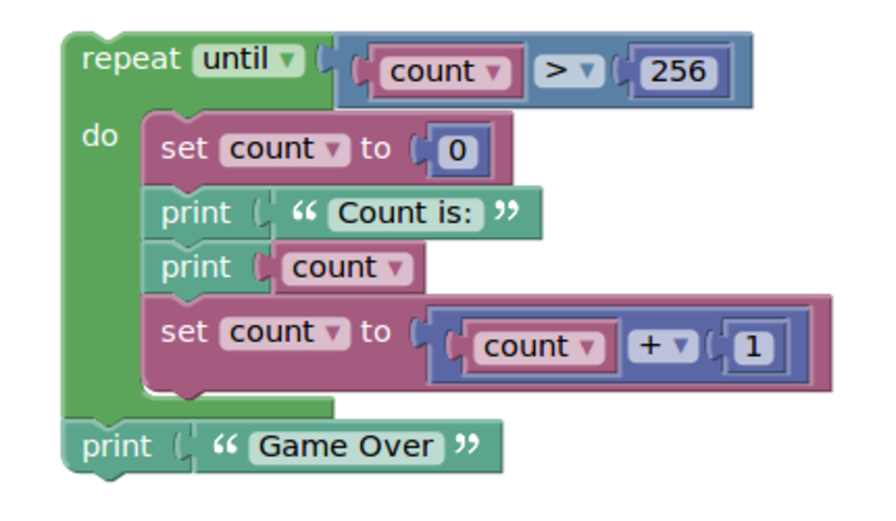
\includegraphics[width=0.5\textwidth]{fig/blockly}
	\caption{Simple program example created in Google's Blockly.}\label{fig:blockly}
\end{figure}

Blockly enables developers to create their own programming environments for their projects, so they
can adapt Blockly itself to their needs, and thus, making it possible for them to even create
complete \acrshort{ide}s for their projects based on visual programming.

\subsection{WebLab-Deusto}

WebLab-Deusto is a remote laboratory facility located in the University of Deusto~\cite{weblab},
Bilbao. Since 2001, it has been providing students with remote laboratories to complete their
academic learnings. Since then, it has been extended and many of it's laboratories is available
all over the world. It's no longer a laboratory only made for microelectronics university students
since nowadays it serves schools and universities everywhere to provide them with remote
laboratories.

Among others, it serves an experiment to prove and measure the Archimedes' principle
(Figure~\ref{fig:archimedes}), an experiment to program and control a robot and some
microelectronics experiments with PLDs and FPGAs. Moreover, there are more laboratories in
development, such as an elevator to teach students how to program and control them, an experiment
with an aquarium where students can give them food and, of course, the project presented here: a
complete learning experience given by a robot.

\begin{figure}[!htbp]
	\centering
	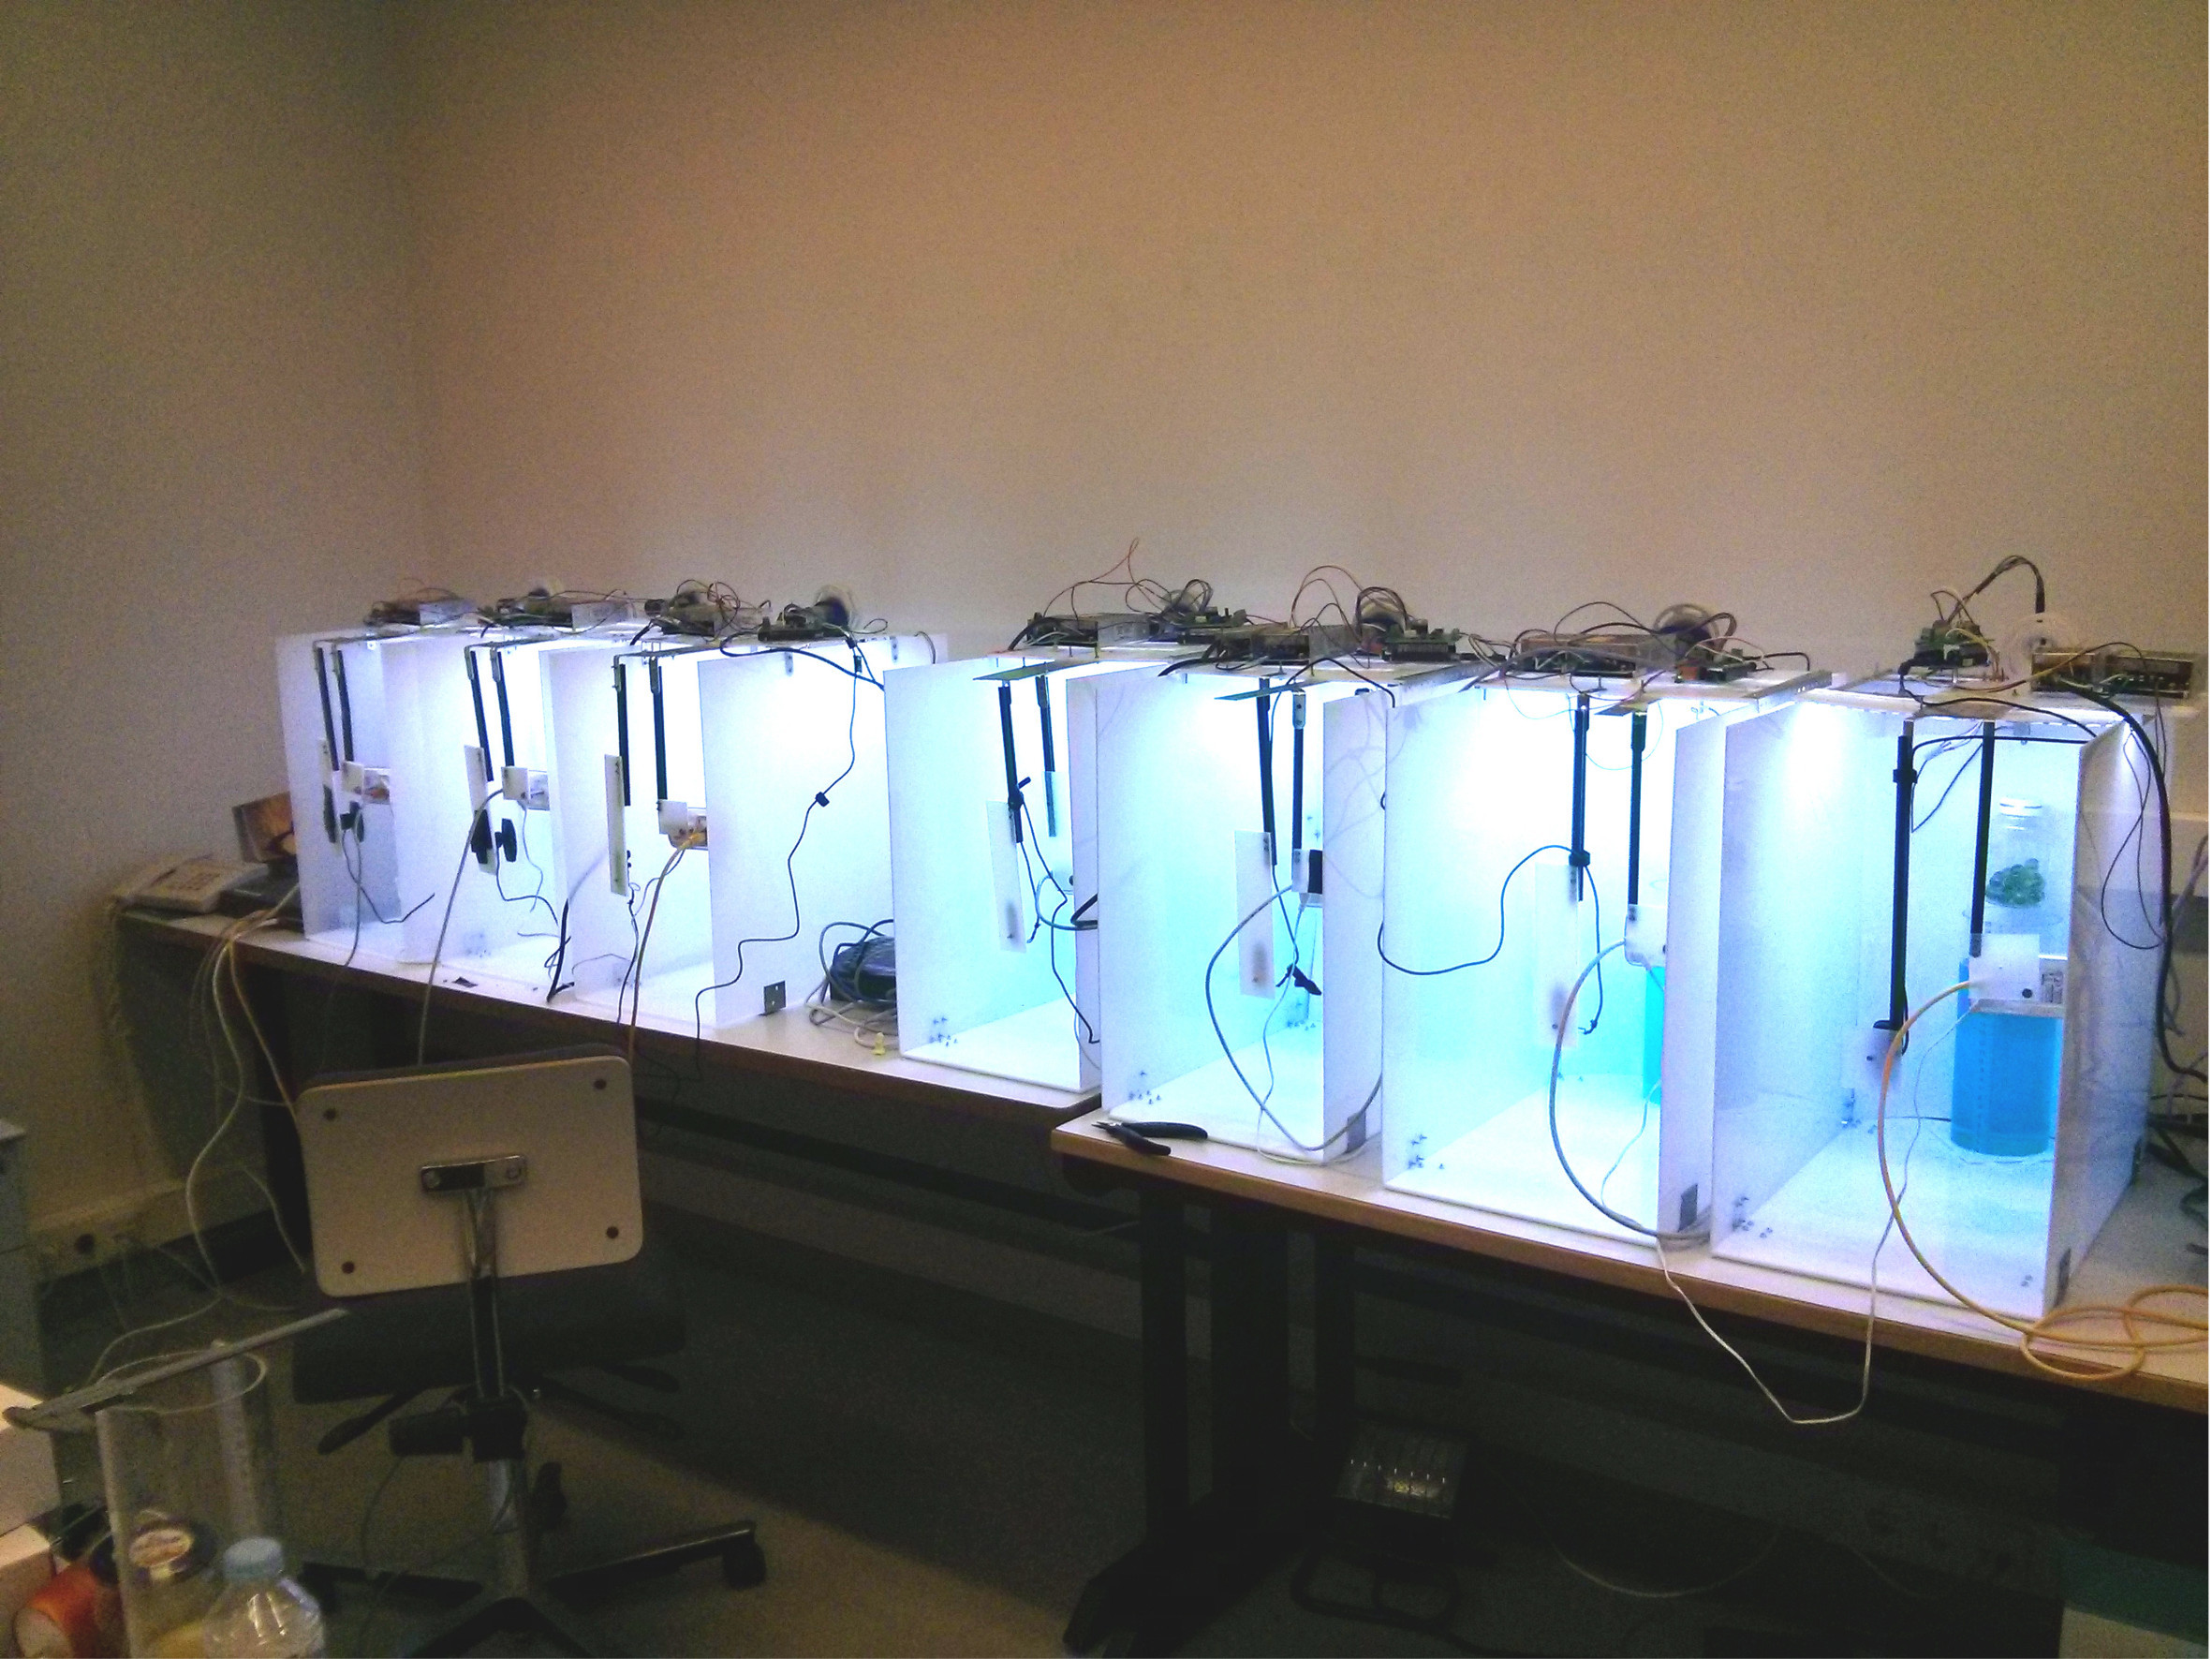
\includegraphics[width=0.5\textwidth]{fig/archimedes}
	\caption{Archimedes experiment in WebLab-Deusto.}\label{fig:archimedes}
\end{figure}

\section{Rationale}

Technology is changing every day, and among other luxuries, it gives us the ability to improve the
way we perform our tasks. Nowadays, one of the most important things in our lives, that consumes
more than a quarter of it is our education. In a strong belief that technology can contribute to
give future generations better tools for learning, serious games seem to be a viable option I would
like to deepen. Having the opportunity to do so in a remote environment such as WebLab-Deusto gives
us the ability to create a remote laboratory, with the potential for being used by many people
around the world, and thus make a difference in learning environments.
